% =============================================================================
%DIF LATEXDIFF DIFFERENCE FILE
%DIF DEL main_twocolumn_SUBMITTED.tex   Mon Jul 27 21:53:31 2026
%DIF ADD main_twocolumn.tex             Mon Jul 27 22:52:52 2026
% PRL variant of the troposwhere manuscript (K=5).
% Reformatted from the Nature-Comp-Sci article-class version
% (preserved in main_natcomp_backup.tex) into REVTeX 4.2 / Physical Review
% Letters format: two-column reprint layout, numeric APS citations
% (apsrev4-2.bst), PRL title/abstract block.
%
% CONVERSION STATUS (pass 1 = reformat; content preserved, not yet cut to
% the PRL length limit ~3750 words / 4 pages):
%   [x] REVTeX 4.2 preamble, prl option, two-column reprint
%   [x] Numeric \cite throughout (was authoryear \citep/\citet)
%   [x] Title / author / affiliation / abstract block
%   [x] Body ported (intro + results + discussion)
%   [x] Methods kept at end (candidate for Supplemental Material / End Matter)
%   [ ] Cut to PRL length (pass 2)
%   [ ] Split heavy Methods -> Supplemental Material (pass 2)
%   [ ] Verify author affiliations (marked TODO below)
% =============================================================================
% Review layout: reprint class (compact title block -> abstract on page 1,
% no empty title page), but the body is forced to a single wide column via
% \onecolumngrid after \maketitle so that line numbers sit cleanly in the
% left margin without the two-column gutter overlap. For the final
% journal-look two-column preview, comment out the \onecolumngrid line below.
\documentclass[
    aps,
    prl,
    reprint,
    superscriptaddress,
    amsmath,amssymb,
    floatfix,
    nofootinbib
]{revtex4-2}

% ── Figures, math, typography ──────────────────────────────────────────
\usepackage{graphicx}
\usepackage{bm}
\usepackage{xcolor}
\usepackage[colorlinks=true,allcolors=blue!50!black,citecolor=blue!50!black]{hyperref}
\usepackage{xr-hyper}                             % cross-refs to Supplemental Material labels
\externaldocument[S]{supplementary}                  % reads supplementary.aux (build SM first)
\usepackage{lineno}                               % line numbers (clean in single-column preprint)
\usepackage{setspace}                             % wider line spacing for the review copy
% \linenumbers is issued after \maketitle (below) to avoid a lineno/REVTeX
% interaction that pushes the abstract onto a blank second page.

\graphicspath{{./}{figures/}{SI_figures/}{img/}}
%DIF PREAMBLE EXTENSION ADDED BY LATEXDIFF
%DIF UNDERLINE PREAMBLE %DIF PREAMBLE
\RequirePackage[normalem]{ulem} %DIF PREAMBLE
\RequirePackage{color}\definecolor{RED}{rgb}{1,0,0}\definecolor{BLUE}{rgb}{0,0,1} %DIF PREAMBLE
\providecommand{\DIFaddtex}[1]{{\protect\color{blue}\uwave{#1}}} %DIF PREAMBLE
\providecommand{\DIFdeltex}[1]{{\protect\color{red}\sout{#1}}} %DIF PREAMBLE
%DIF SAFE PREAMBLE %DIF PREAMBLE
\providecommand{\DIFaddbegin}{} %DIF PREAMBLE
\providecommand{\DIFaddend}{} %DIF PREAMBLE
\providecommand{\DIFdelbegin}{} %DIF PREAMBLE
\providecommand{\DIFdelend}{} %DIF PREAMBLE
\providecommand{\DIFmodbegin}{} %DIF PREAMBLE
\providecommand{\DIFmodend}{} %DIF PREAMBLE
%DIF FLOATSAFE PREAMBLE %DIF PREAMBLE
\providecommand{\DIFaddFL}[1]{\DIFadd{#1}} %DIF PREAMBLE
\providecommand{\DIFdelFL}[1]{\DIFdel{#1}} %DIF PREAMBLE
\providecommand{\DIFaddbeginFL}{} %DIF PREAMBLE
\providecommand{\DIFaddendFL}{} %DIF PREAMBLE
\providecommand{\DIFdelbeginFL}{} %DIF PREAMBLE
\providecommand{\DIFdelendFL}{} %DIF PREAMBLE
%DIF HYPERREF PREAMBLE %DIF PREAMBLE
\providecommand{\DIFadd}[1]{\texorpdfstring{\DIFaddtex{#1}}{#1}} %DIF PREAMBLE
\providecommand{\DIFdel}[1]{\texorpdfstring{\DIFdeltex{#1}}{}} %DIF PREAMBLE
\providecommand{\DIFscaledelfig}{0.5}
%DIF HIGHLIGHTGRAPHICS PREAMBLE %DIF PREAMBLE
\RequirePackage{settobox} %DIF PREAMBLE
\RequirePackage{letltxmacro} %DIF PREAMBLE
\newsavebox{\DIFdelgraphicsbox} %DIF PREAMBLE
\newlength{\DIFdelgraphicswidth} %DIF PREAMBLE
\newlength{\DIFdelgraphicsheight} %DIF PREAMBLE
% store original definition of \includegraphics %DIF PREAMBLE
\LetLtxMacro{\DIFOincludegraphics}{\includegraphics} %DIF PREAMBLE
\providecommand{\DIFaddincludegraphics}[2][]{{\color{blue}\fbox{\DIFOincludegraphics[#1]{#2}}}} %DIF PREAMBLE
\providecommand{\DIFdelincludegraphics}[2][]{% %DIF PREAMBLE
\sbox{\DIFdelgraphicsbox}{\DIFOincludegraphics[#1]{#2}}% %DIF PREAMBLE
\settoboxwidth{\DIFdelgraphicswidth}{\DIFdelgraphicsbox} %DIF PREAMBLE
\settoboxtotalheight{\DIFdelgraphicsheight}{\DIFdelgraphicsbox} %DIF PREAMBLE
\scalebox{\DIFscaledelfig}{% %DIF PREAMBLE
\parbox[b]{\DIFdelgraphicswidth}{\usebox{\DIFdelgraphicsbox}\\[-\baselineskip] \rule{\DIFdelgraphicswidth}{0em}}\llap{\resizebox{\DIFdelgraphicswidth}{\DIFdelgraphicsheight}{% %DIF PREAMBLE
\setlength{\unitlength}{\DIFdelgraphicswidth}% %DIF PREAMBLE
\begin{picture}(1,1)% %DIF PREAMBLE
\thicklines\linethickness{2pt} %DIF PREAMBLE
{\color[rgb]{1,0,0}\put(0,0){\framebox(1,1){}}}% %DIF PREAMBLE
{\color[rgb]{1,0,0}\put(0,0){\line( 1,1){1}}}% %DIF PREAMBLE
{\color[rgb]{1,0,0}\put(0,1){\line(1,-1){1}}}% %DIF PREAMBLE
\end{picture}% %DIF PREAMBLE
}\hspace*{3pt}}} %DIF PREAMBLE
} %DIF PREAMBLE
\LetLtxMacro{\DIFOaddbegin}{\DIFaddbegin} %DIF PREAMBLE
\LetLtxMacro{\DIFOaddend}{\DIFaddend} %DIF PREAMBLE
\LetLtxMacro{\DIFOdelbegin}{\DIFdelbegin} %DIF PREAMBLE
\LetLtxMacro{\DIFOdelend}{\DIFdelend} %DIF PREAMBLE
\DeclareRobustCommand{\DIFaddbegin}{\DIFOaddbegin \let\includegraphics\DIFaddincludegraphics} %DIF PREAMBLE
\DeclareRobustCommand{\DIFaddend}{\DIFOaddend \let\includegraphics\DIFOincludegraphics} %DIF PREAMBLE
\DeclareRobustCommand{\DIFdelbegin}{\DIFOdelbegin \let\includegraphics\DIFdelincludegraphics} %DIF PREAMBLE
\DeclareRobustCommand{\DIFdelend}{\DIFOaddend \let\includegraphics\DIFOincludegraphics} %DIF PREAMBLE
\LetLtxMacro{\DIFOaddbeginFL}{\DIFaddbeginFL} %DIF PREAMBLE
\LetLtxMacro{\DIFOaddendFL}{\DIFaddendFL} %DIF PREAMBLE
\LetLtxMacro{\DIFOdelbeginFL}{\DIFdelbeginFL} %DIF PREAMBLE
\LetLtxMacro{\DIFOdelendFL}{\DIFdelendFL} %DIF PREAMBLE
\DeclareRobustCommand{\DIFaddbeginFL}{\DIFOaddbeginFL \let\includegraphics\DIFaddincludegraphics} %DIF PREAMBLE
\DeclareRobustCommand{\DIFaddendFL}{\DIFOaddendFL \let\includegraphics\DIFOincludegraphics} %DIF PREAMBLE
\DeclareRobustCommand{\DIFdelbeginFL}{\DIFOdelbeginFL \let\includegraphics\DIFdelincludegraphics} %DIF PREAMBLE
\DeclareRobustCommand{\DIFdelendFL}{\DIFOaddendFL \let\includegraphics\DIFOincludegraphics} %DIF PREAMBLE
%DIF AMSMATHULEM PREAMBLE %DIF PREAMBLE
\makeatletter %DIF PREAMBLE
\let\sout@orig\sout %DIF PREAMBLE
\renewcommand{\sout}[1]{\ifmmode\text{\sout@orig{\ensuremath{#1}}}\else\sout@orig{#1}\fi} %DIF PREAMBLE
\makeatother %DIF PREAMBLE
%DIF COLORLISTINGS PREAMBLE %DIF PREAMBLE
\RequirePackage{listings} %DIF PREAMBLE
\RequirePackage{color} %DIF PREAMBLE
\lstdefinelanguage{DIFcode}{ %DIF PREAMBLE
%DIF DIFCODE_UNDERLINE %DIF PREAMBLE
  moredelim=[il][\color{red}\sout]{\%DIF\ <\ }, %DIF PREAMBLE
  moredelim=[il][\color{blue}\uwave]{\%DIF\ >\ } %DIF PREAMBLE
} %DIF PREAMBLE
\lstdefinestyle{DIFverbatimstyle}{ %DIF PREAMBLE
	language=DIFcode, %DIF PREAMBLE
	basicstyle=\ttfamily, %DIF PREAMBLE
	columns=fullflexible, %DIF PREAMBLE
	keepspaces=true %DIF PREAMBLE
} %DIF PREAMBLE
\lstnewenvironment{DIFverbatim}[1][]{\lstset{style=DIFverbatimstyle}}{} %DIF PREAMBLE
\lstnewenvironment{DIFverbatim*}[1][]{\lstset{style=DIFverbatimstyle,showspaces=true}}{} %DIF PREAMBLE
\lstset{extendedchars=\true,inputencoding=utf8}

%DIF END PREAMBLE EXTENSION ADDED BY LATEXDIFF

\begin{document}

\title{A temporally-constrained latent space reveals \\ 
the stochastic dynamics of convective organization}

\author{Sophie Abramian}
\affiliation{Department of Earth and Environmental Engineering, Columbia University, New York, NY, USA}

\author{Olivier Pauluis}
\affiliation{Courant Institute of Mathematical Sciences, New York University, New York, NY, USA}

\author{L. Ruby Leung}
\affiliation{Atmospheric Sciences and Global Change Division, Pacific Northwest National Laboratory, Richland, WA, USA}


\author{Pierre Gentine}
\affiliation{Department of Earth and Environmental Engineering, Columbia University, New York, NY, USA}




\date{\today}

\begin{abstract}
Atmospheric convection is intrinsically stochastic: under identical large-scale forcing, storms can follow widely different life cycles. We introduce an unsupervised framework that learns a low-dimensional representation of cloud-resolving squall-line simulations by constraining the latent space to evolve according to a linear stochastic operator. The learned representation partitions convection into five physically interpretable states whose transitions define a Markov chain. Its spectrum reveals a dominant slow mode separating organized from unorganized convection and governing the system's life cycle. The remaining departures from Markovianity are partly explained by cold pools, identifying a physical source of memory absent from the reduced description. The framework provides a physically interpretable stochastic coarse-graining of convection and offers an alternative to existing multi-cloud parameterizations.
\end{abstract}

\maketitle

% ── Introduction (no heading, PRL Letter style) ────────────────────────
Discovering interpretable, low-dimensional representations of high-dimensional stochastic \DIFdelbegin \DIFdel{dynamics }\DIFdelend \DIFaddbegin \DIFadd{systems }\DIFaddend is a foundational challenge across the physical sciences. Deep convection \DIFdelbegin \DIFdel{in the atmosphere }\DIFdelend is a prime example\DIFdelbegin \DIFdel{. Deep }\DIFdelend \DIFaddbegin \DIFadd{: deep }\DIFaddend convective systems---organized cloud structures larger and longer-lived than individual cells---dominate the tropical water and energy cycle \cite{houze2004mesoscale, chakraborty2023overview}; the largest \DIFdelbegin \DIFdel{, mesoscale convective systems, }\DIFdelend contribute over 50\% of tropical precipitation and a disproportionate share of extremes \cite{roca2020extreme, feng2024mesoscale, feng2023mesoscale}.

In climate models they occur below the grid scale and must be \DIFdelbegin \DIFdel{parameterized---a }\DIFdelend \DIFaddbegin \DIFadd{parameterized, a }\DIFaddend persistent source of uncertainty \DIFdelbegin \DIFdel{, especially }\DIFdelend under warming \cite{yang2023impact, bolot2025no}. The difficulty is that a convective system is \DIFdelbegin \DIFdel{a }\DIFdelend high-dimensional\DIFdelbegin \DIFdel{dynamical object; }\DIFdelend \DIFaddbegin \DIFadd{: }\DIFaddend compressing it into a few prognostic variables without discarding what matters is hard.

Compounding this, \DIFdelbegin \DIFdel{the convective response to a }\DIFdelend \DIFaddbegin \DIFadd{under }\DIFaddend \emph{fixed} large-scale forcing \DIFaddbegin \DIFadd{the convective response }\DIFaddend is not a single outcome but a broad distribution of storm evolutions \cite{abramian2025key, feng2025mesoscale, hu2020observed, fiolleau2024database}---an \emph{internal} variability intrinsic to \DIFdelbegin \DIFdel{the convection, not inherited from the environment}\DIFdelend \DIFaddbegin \DIFadd{convection}\DIFaddend . Capturing it requires a reduced description \DIFdelbegin \DIFdel{that is }\DIFdelend both low-dimensional and faithful to the dynamics.

Stochastic multi-cloud models \cite{khouider2006multicloud, majda2008stochastic, khouider2010stochastic} offer such a reduction, but \DIFdelbegin \DIFdel{a strongly simplified }\DIFdelend one whose states are prescribed \emph{a priori}: a lattice of sites, each in one of a few hand-chosen cloud states---clear sky, shallow, congestus, or deep---whose area fractions evolve by a Markov chain. This captures the changing cloud cover but not the vertical mass-flux profiles that also govern extreme precipitation \cite{MullerYukari19, singh2012upward, abramian2023extreme, wang2022convective, li2025bimodal}.

Koopman operator theory \cite{koopman1931hamiltonian, brunton2021modern} offers a principled alternative. Instead of the state $\mathbf{x}_t$ of a high-dimensional nonlinear system, one follows \emph{observables} $g(\mathbf{x})$ that recast it in new coordinates; the operator advancing them---$\mathcal{K}$, the Koopman operator, defined by $(\mathcal{K}g)(\mathbf{x}_t) = g(\mathbf{x}_{t+1})$---is linear by construction, whatever the nonlinear dynamics. The challenge is \DIFdelbegin \DIFdel{thus }\DIFdelend \DIFaddbegin \DIFadd{then }\DIFaddend not to resolve the nonlinear evolution \DIFdelbegin \DIFdel{, }\DIFdelend but to find an observable that simplifies \DIFdelbegin \DIFdel{it---ideally one on which $\mathcal{K}$ acts as a simple multiplication---while }\DIFdelend \DIFaddbegin \DIFadd{it while }\DIFaddend retaining most of the system's information. Such an observable is generally infinite-dimensional \cite{brunton2021modern}---the long-standing obstacle. Only recently have machine-learning encoder--decoder architectures \cite{lusch2018deep, nathaniel2026generative} overcome it, learning from data the best finite-dimensional observable for a given latent dimension together with its linear operator.

We depart from existing Koopman autoencoders in two ways. First, we start from a physically reduced representation\DIFdelbegin \DIFdel{of the system}\DIFdelend , casting the flow in isentropic coordinates \cite{pauluis2013isentropic}---a thermodynamically consistent reduction that filters reversible adiabatic motions---rather than \DIFdelbegin \DIFdel{using the raw , noisy }\DIFdelend \DIFaddbegin \DIFadd{raw }\DIFaddend three-dimensional fields. Second, rather than enforcing \emph{deterministic} linear dynamics, we \emph{partition} the latent space into discrete states by joint clustering \cite{kaiser2014cluster, souza2024representing} and model their transitions \emph{probabilistically}. The result is a Markov chain \DIFdelbegin \DIFdel{on data-discovered states---finite-dimensional, stochastic, and shaped by the dynamics it represents}\DIFdelend \DIFaddbegin \DIFadd{whose states are discovered from the data rather than prescribed}\DIFaddend . Though demonstrated on convection, the framework applies to any high-dimensional system where regime discovery and transition modeling are needed.

We analyze cloud-resolving simulations of squall lines (SAM~\cite{khairoutdinov2003}) under fixed vertical wind shear, in statistical equilibrium yet with strong internal variability. \DIFdelbegin \DIFdel{Convection is cast in isentropic coordinates: at }\DIFdelend \DIFaddbegin \DIFadd{At }\DIFaddend each time the three-dimensional vertical mass flux is projected onto height $z$ and moist static energy $h$, yielding a two-dimensional diagram $M(h,z)$ that \DIFdelbegin \DIFdel{cleanly }\DIFdelend separates high-$h$ updrafts from the low-$h$ evaporative downdrafts that build cold pools~\cite{pauluis2013isentropic}. Figure~\ref{fig:simu_isentrop} shows three representative \DIFdelbegin \DIFdel{snapshots---suppressed, organized-deep, and unorganized-active convection---alongside }\DIFdelend \DIFaddbegin \DIFadd{snapshots alongside }\DIFaddend their mass-flux diagrams; this time series \DIFdelbegin \DIFdel{of diagrams }\DIFdelend is the input to the model.

\begin{figure}[t]
    \centering
    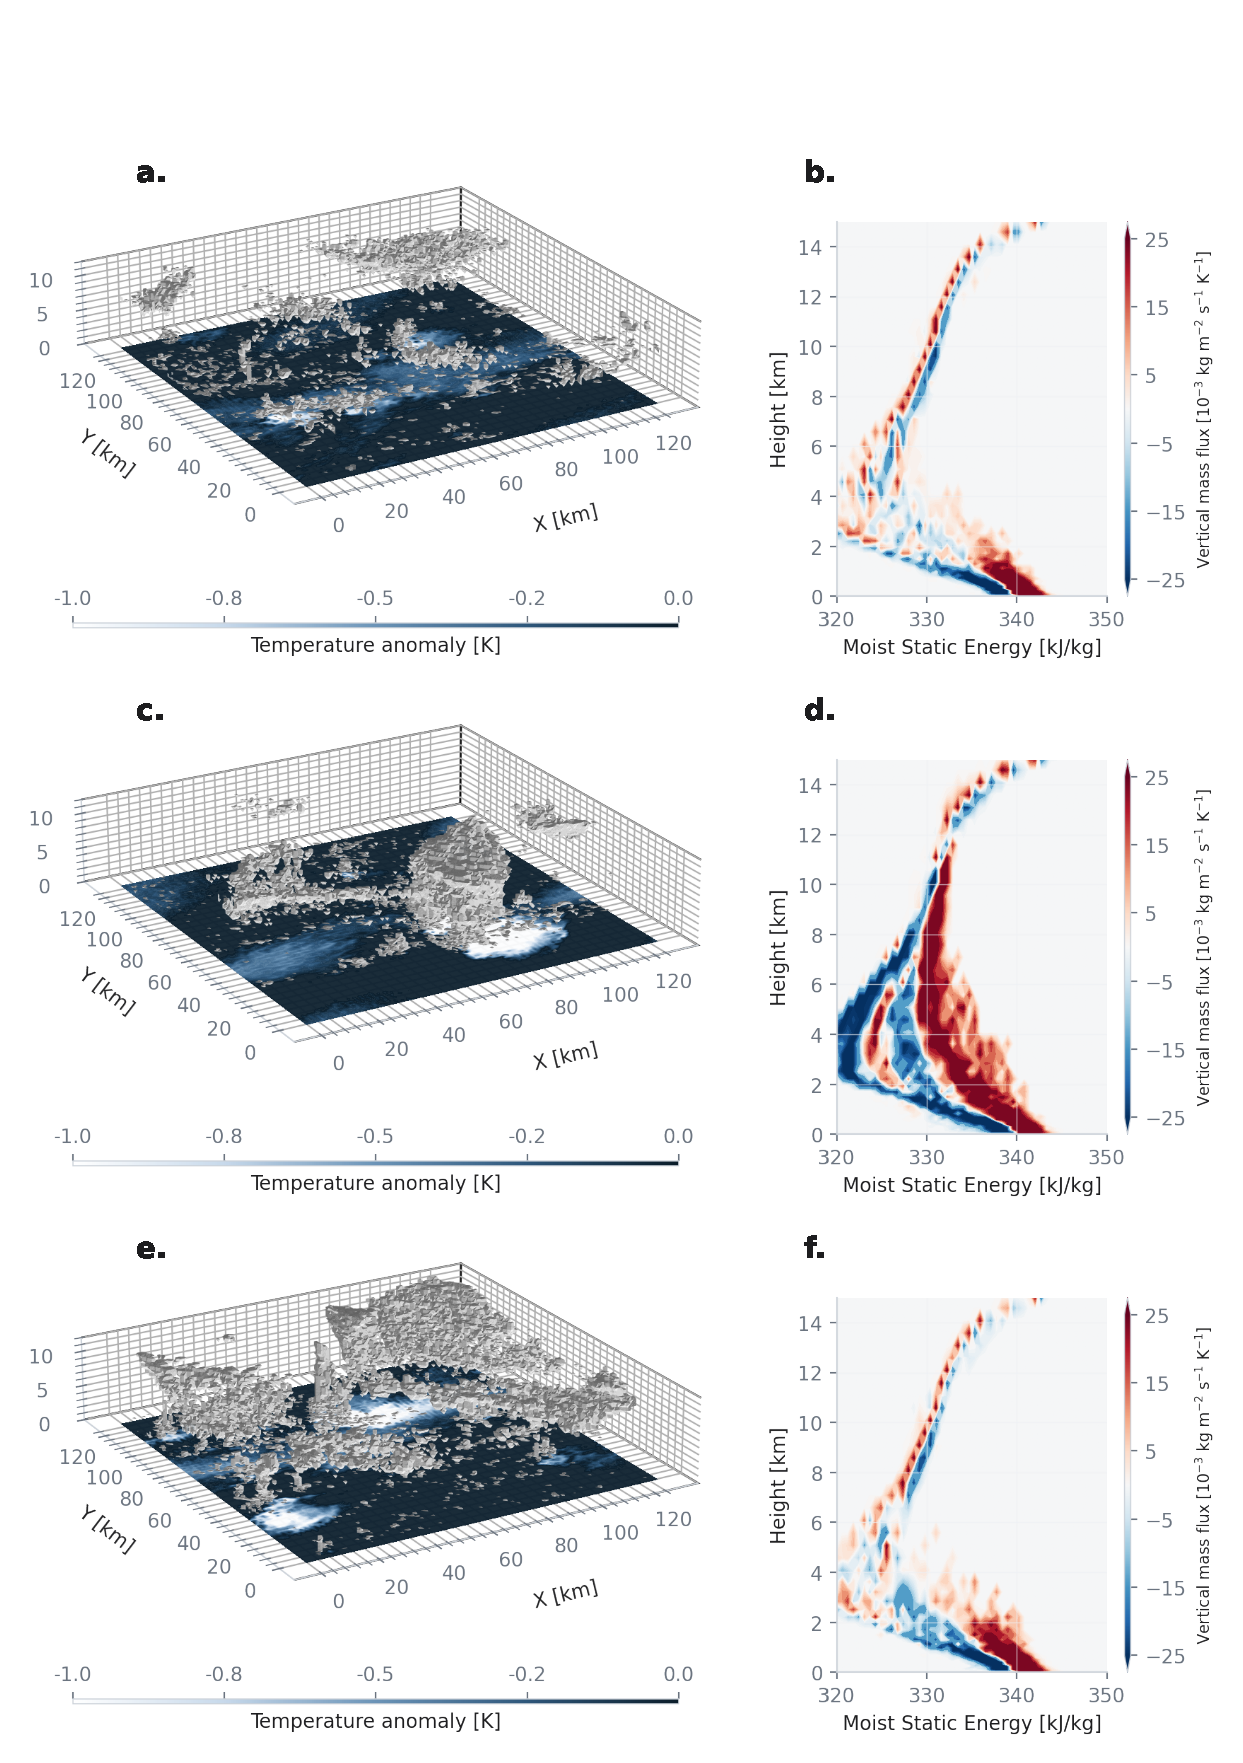
\includegraphics[width=\columnwidth]{fig1_snapshots.pdf}
    \caption{\DIFdelbeginFL \textbf{\DIFdelFL{Three contrasting snapshots of the simulated convective field.}} %DIFAUXCMD
\DIFdelendFL \DIFaddbeginFL \textbf{\DIFaddFL{Three contrasting snapshots of the convective field.}} \DIFaddendFL \textbf{Left (a, c, e):} isovolume of non-precipitating condensate $\mathrm{QN}=0.02$~kg\,kg$^{-1}$ over the surface temperature anomaly; white patches mark cold pools. \textbf{Right (b, d, f):} \DIFdelbeginFL \DIFdelFL{the corresponding }\DIFdelendFL isentropic mass-flux diagram $M(h,z,t)$, red (blue) for upward (downward) transport. Rows: \textbf{(a--b)} suppressed, \textbf{(c--d)} organized deep, \DIFdelbeginFL \DIFdelFL{and }\DIFdelendFL \textbf{(e--f)} unorganized active\DIFdelbeginFL \DIFdelFL{convection}\DIFdelendFL .}
    \label{fig:simu_isentrop}
\end{figure}

Applied to these simulations, the construction asks: (i)\DIFaddbegin \DIFadd{~}\DIFaddend what mass-flux states a given forcing makes accessible; (ii)\DIFaddbegin \DIFadd{~}\DIFaddend whether their transitions form a Markov chain, and how organized and weakly organized pathways differ; (iii)\DIFaddbegin \DIFadd{~}\DIFaddend where internal feedbacks---cold pools in particular---introduce memory beyond the discrete state. Five interpretable states emerge without supervision, and their transitions form a Markov chain with a slow ($\sim$3\,h) eigenmode alternating two regimes, organized and unorganized; two long-lived states decay more slowly than their Markov prediction, and conditioning on cold-pool intensity closes $\sim$30\% of that gap.

% ── Results ────────────────────────────────────────────────────────────
\section{Construction and physical interpretation of the latent space}

The squall-line evolution is seen through its time series of isentropic mass-flux fields $X_t$. \DIFdelbegin \DIFdel{The model compresses each field into a latent vector $\mathbf{z}_t\in\mathbb{R}^8$ and groups it into five discrete states. Specifically, an }\DIFdelend \DIFaddbegin \DIFadd{An }\DIFaddend encoder maps $X_t$ to a Gaussian posterior over \DIFdelbegin \DIFdel{$\mathbf{z}_t$ }\DIFdelend \DIFaddbegin \DIFadd{a latent vector $\mathbf{z}_t\in\mathbb{R}^8$ }\DIFaddend (a variational autoencoder with reconstruction and Kullback--Leibler terms); a softmax head turns $\mathbf{z}_t$ into a probability vector $s_t$ over \DIFdelbegin \DIFdel{the }\DIFdelend $K=5$ states; and a row-stochastic matrix $\mathbf{T}$ propagates it one step, $s_{t+1}\approx\mathbf{T}\,s_t$. \DIFdelbegin \DIFdel{These three components }\DIFdelend \DIFaddbegin \DIFadd{The three }\DIFaddend are trained jointly on consecutive pairs $(X_t, X_{t+\Delta t})$, so the latent space is at once reconstructive, cluster-separable, and dynamically predictive (Fig.~\ref{fig:model}). A contrastive \DIFdelbegin \DIFdel{loss based on the structural }\DIFdelend (Dice) \DIFdelbegin \DIFdel{similarity of }\DIFdelend \DIFaddbegin \DIFadd{loss on }\DIFaddend the mass-flux fields prevents state collapse, keeping all five states populated. Full \DIFdelbegin \DIFdel{architecture, losses, and training are given }\DIFdelend \DIFaddbegin \DIFadd{details are }\DIFaddend in the Supplemental Material.

\begin{figure}[!ht]
    \centering
    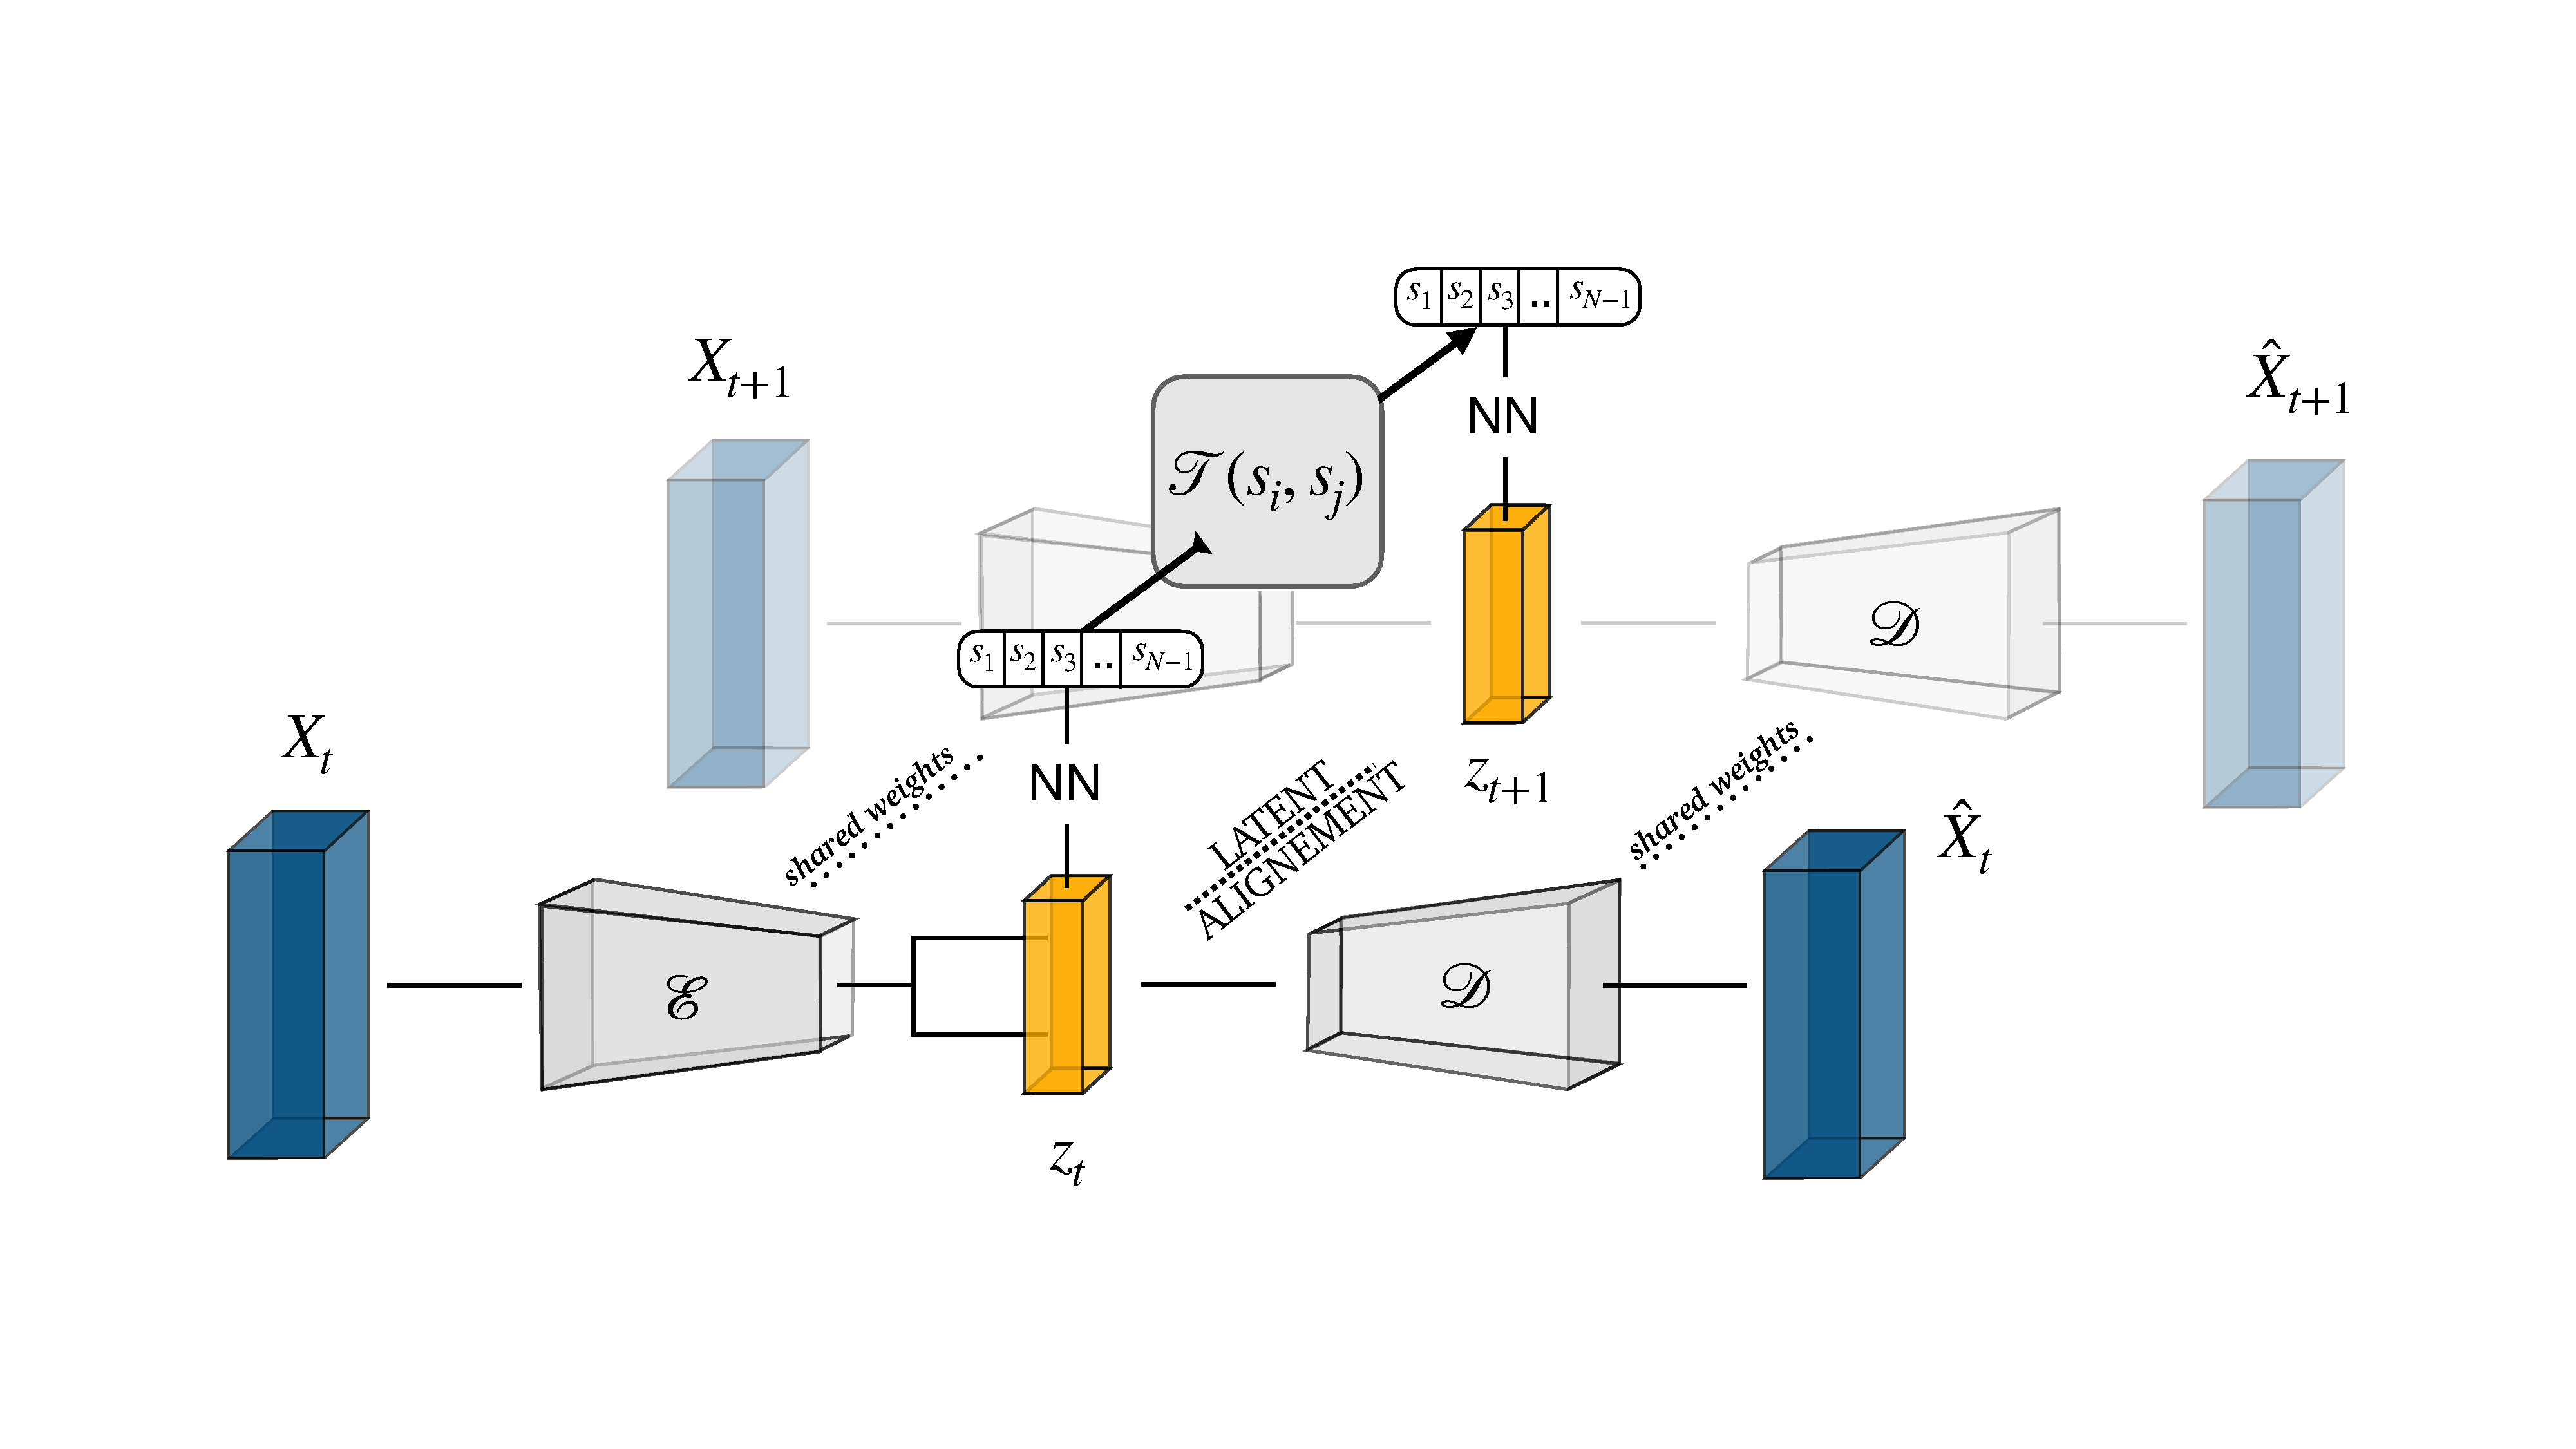
\includegraphics[width=\columnwidth]{model_vae_mc.pdf}
    \caption{\textbf{Model architecture.} A variational autoencoder \DIFdelbeginFL \DIFdelFL{(VAE) }\DIFdelendFL is coupled to a Markovian state-assignment and transition framework \DIFdelbeginFL \DIFdelFL{. An encoder maps the input to a latent representation $z_t$, reconstructed by a decoder; a small network assigns each $z_t$ a probability distribution over $K=5$ discrete states; }\DIFdelendFL and \DIFdelbeginFL \DIFdelFL{a linear transition operator $T$ predicts }\DIFdelendFL \DIFaddbeginFL \DIFaddFL{trained jointly (components defined in }\DIFaddendFL the \DIFdelbeginFL \DIFdelFL{state distribution at $t+1$ from that at $t$}\DIFdelendFL \DIFaddbeginFL \DIFaddFL{text)}\DIFaddendFL .}
    \label{fig:model}
\end{figure}

No physical constraint is imposed during \DIFdelbegin \DIFdel{training---the }\DIFdelend \DIFaddbegin \DIFadd{training: the }\DIFaddend VAE is regularized only toward an isotropic Gaussian \DIFdelbegin \DIFdel{, }\DIFdelend and states are assigned without reference to \DIFdelbegin \DIFdel{intensity, organization, or any diagnostic---so whether the }\DIFdelend \DIFaddbegin \DIFadd{any physical diagnostic, so a physically meaningful }\DIFaddend latent space is \DIFdelbegin \DIFdel{physically meaningful is }\DIFdelend not guaranteed. Applying PCA to $\mathbf{z}(t)$, the first two components explain $22\%$ and $17\%$ of the variance (Fig.~\ref{fig:clusters}); a three-dimensional projection (Supplemental Material, Fig.~\ref{Sfig:pca_3d}) shows that states overlapping in 2D separate along higher-order components.

\begin{figure*}[t]
    \centering
    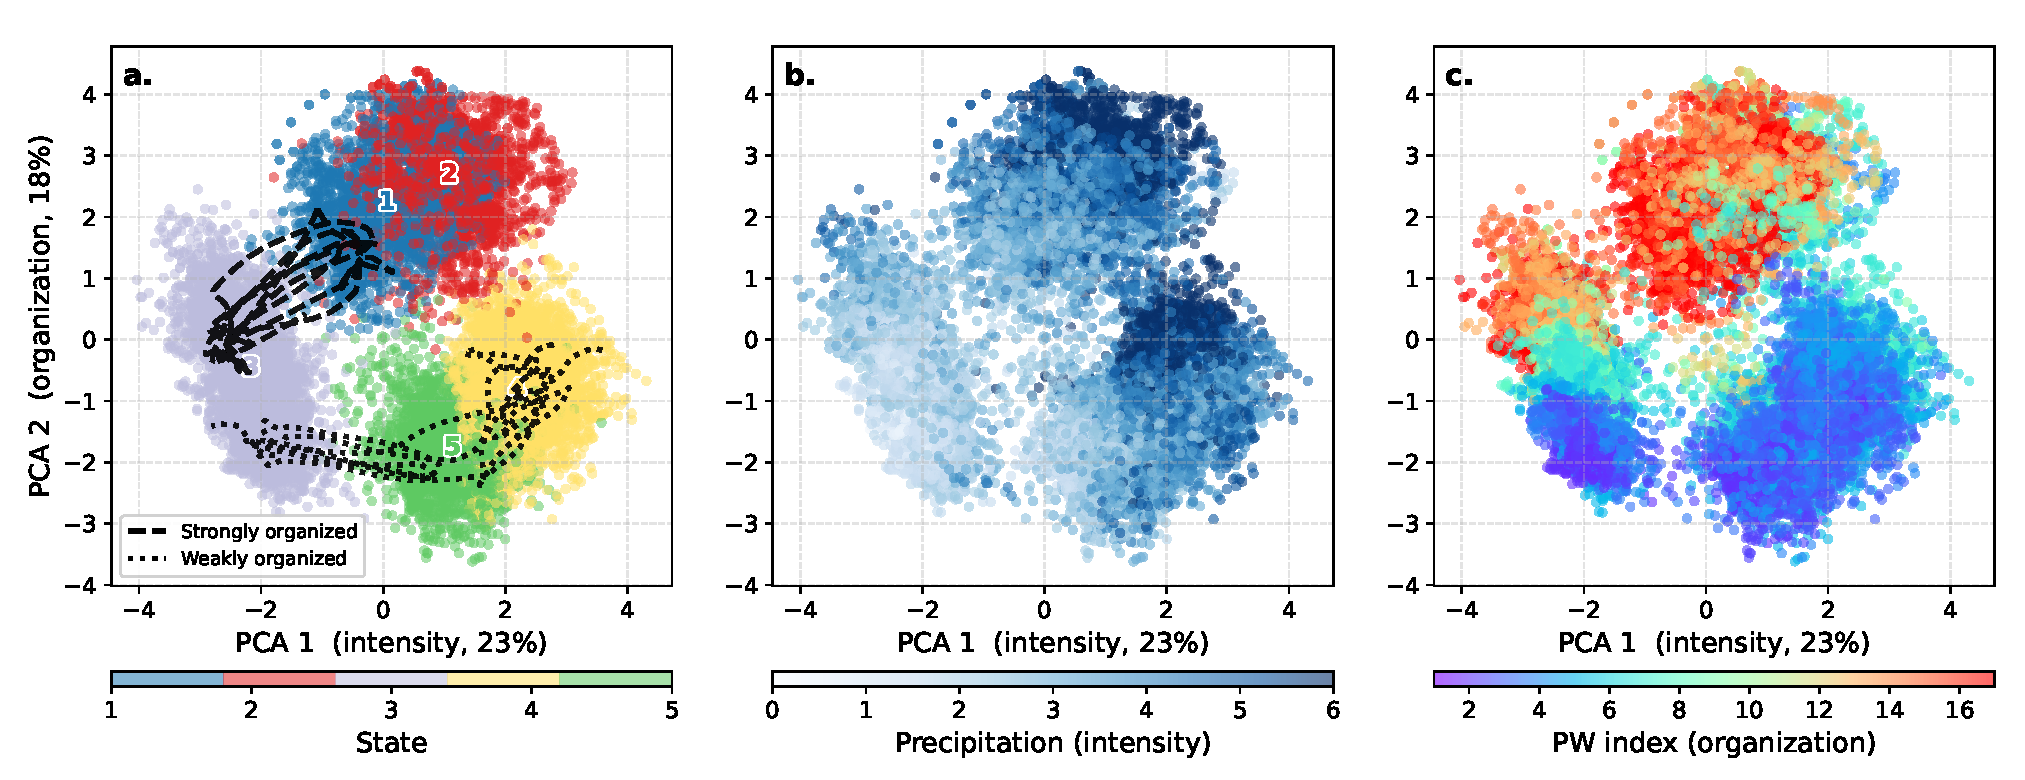
\includegraphics[width=0.98\textwidth]{fig_pca_panels.pdf}
    \caption{\textbf{Latent-space visualization and physical interpretation.} PCA projection of the latent space (each point is one time step), coloured by \textbf{(a)}~state assignment, with two example trajectories over 5~h (dashed: strongly organized; dotted: weakly organized\DIFdelbeginFL \DIFdelFL{; time series in the Supplemental Material}\DIFdelendFL ); \textbf{(b)}~domain-mean precipitation, a proxy for convective intensity; and \textbf{(c)}~the variance of precipitable water (the PW index), a proxy for spatial organization (higher values indicate more clustered convection). \DIFdelbeginFL \DIFdelFL{The first component (PCA~1) aligns with intensity, the second (PCA~2) with organization; joint }\DIFdelendFL \DIFaddbeginFL \DIFaddFL{Joint }\DIFaddendFL distributions \DIFdelbeginFL \DIFdelFL{of the two components against these diagnostics }\DIFdelendFL are given in the Supplemental Material (Fig.~\ref{Sfig:axis_var}).}
    \label{fig:clusters}
\end{figure*}

The dominant latent directions are physically interpretable (Fig.~\ref{fig:clusters}). The first principal component correlates strongly with domain-mean precipitation---convective intensity and life-cycle stage, from suppressed to vigorously precipitating. The second is nearly uncorrelated with precipitation but strongly anticorrelated with the variance of precipitable water, a proxy for spatial organization. Intensity and organization thus emerge as two largely independent axes of the learned representation.

The five states are also dynamically and thermodynamically distinct. Averaging the isentropic mass flux within each state as anomalies from the simulation-wide mean (definitions and full profiles in the Supplemental Material) shows that the organized-deep and stratiform-like states carry deep, high--moist-static-energy \DIFdelbegin \DIFdel{ascent---the stratiform-like state additionally showing a mid-level mass-flux signature suggestive of stratiform detrainment---while }\DIFdelend \DIFaddbegin \DIFadd{ascent, while }\DIFaddend the active-unorganized state peaks at lower altitude and lower moist static energy, and the suppressed and shallow-congestus states carry only weak, shallow anomalies. Table~\ref{tab:state_summary} summarizes each state.

\begin{table*}[t]
\centering
\begin{ruledtabular}
\begin{tabular}{c l c p{0.42\textwidth}}
State & Name & $\pi$ (\%) & Physical signature \\
\hline
1 & \emph{Organized deep}     & 12.9 & sustained deep ascent in a moist environment; reduced low-level detrainment; highest precipitable-water variance \\
2 & \emph{Stratiform-like}    & 12.2 & strongly active convection with large upper-tropospheric mass flux, consistent with a mesoscale stratiform region; highest precipitation \\
3 & \emph{Suppressed convection} & 37.0 & weak up- and down-drafts; dry background atmosphere; dominant state \\
4 & \emph{Active unorganized}     & 22.7 & active but unorganized convection, with mass flux peaking at lower altitudes than in the organized regime; drier environment \\
5 & \emph{Shallow congestus}      & 15.2 & suppressed deep convection with residual shallow convective activity; dry environment \\
\end{tabular}
\end{ruledtabular}
\caption{\textbf{Summary of the five latent convective states.} \DIFdelbeginFL \DIFdelFL{State identities }\DIFdelendFL \DIFaddbeginFL \DIFaddFL{Identities }\DIFaddendFL are inferred from the latent-space axes \DIFdelbeginFL \DIFdelFL{of variability }\DIFdelendFL (Fig.~\ref{fig:clusters}) and confirmed by \DIFdelbeginFL \DIFdelFL{the }\DIFdelendFL per-state \DIFdelbeginFL \DIFdelFL{vertical and moist-static-energy }\DIFdelendFL mass-flux profiles (Supplemental Material). $\pi_i$ is the stationary probability of state~$i$ [Eq.~\eqref{eq:canon}].}
\label{tab:state_summary}
\end{table*}

\section{Markov transition matrix, eigenmodes, and regimes}

The second output of the model is a Markov transition matrix $\mathbf{T}$, whose elements
\begin{equation}
T_{ij} = \mathbb{P}\left( X_{t+\Delta t} = j \mid X_t = i \right)
\end{equation}
denote the probability of transitioning from state $i$ to state $j$. The resulting transition matrix is shown in Fig.~\ref{fig:markov_matrix}.

\begin{figure*}[t]
    \centering
    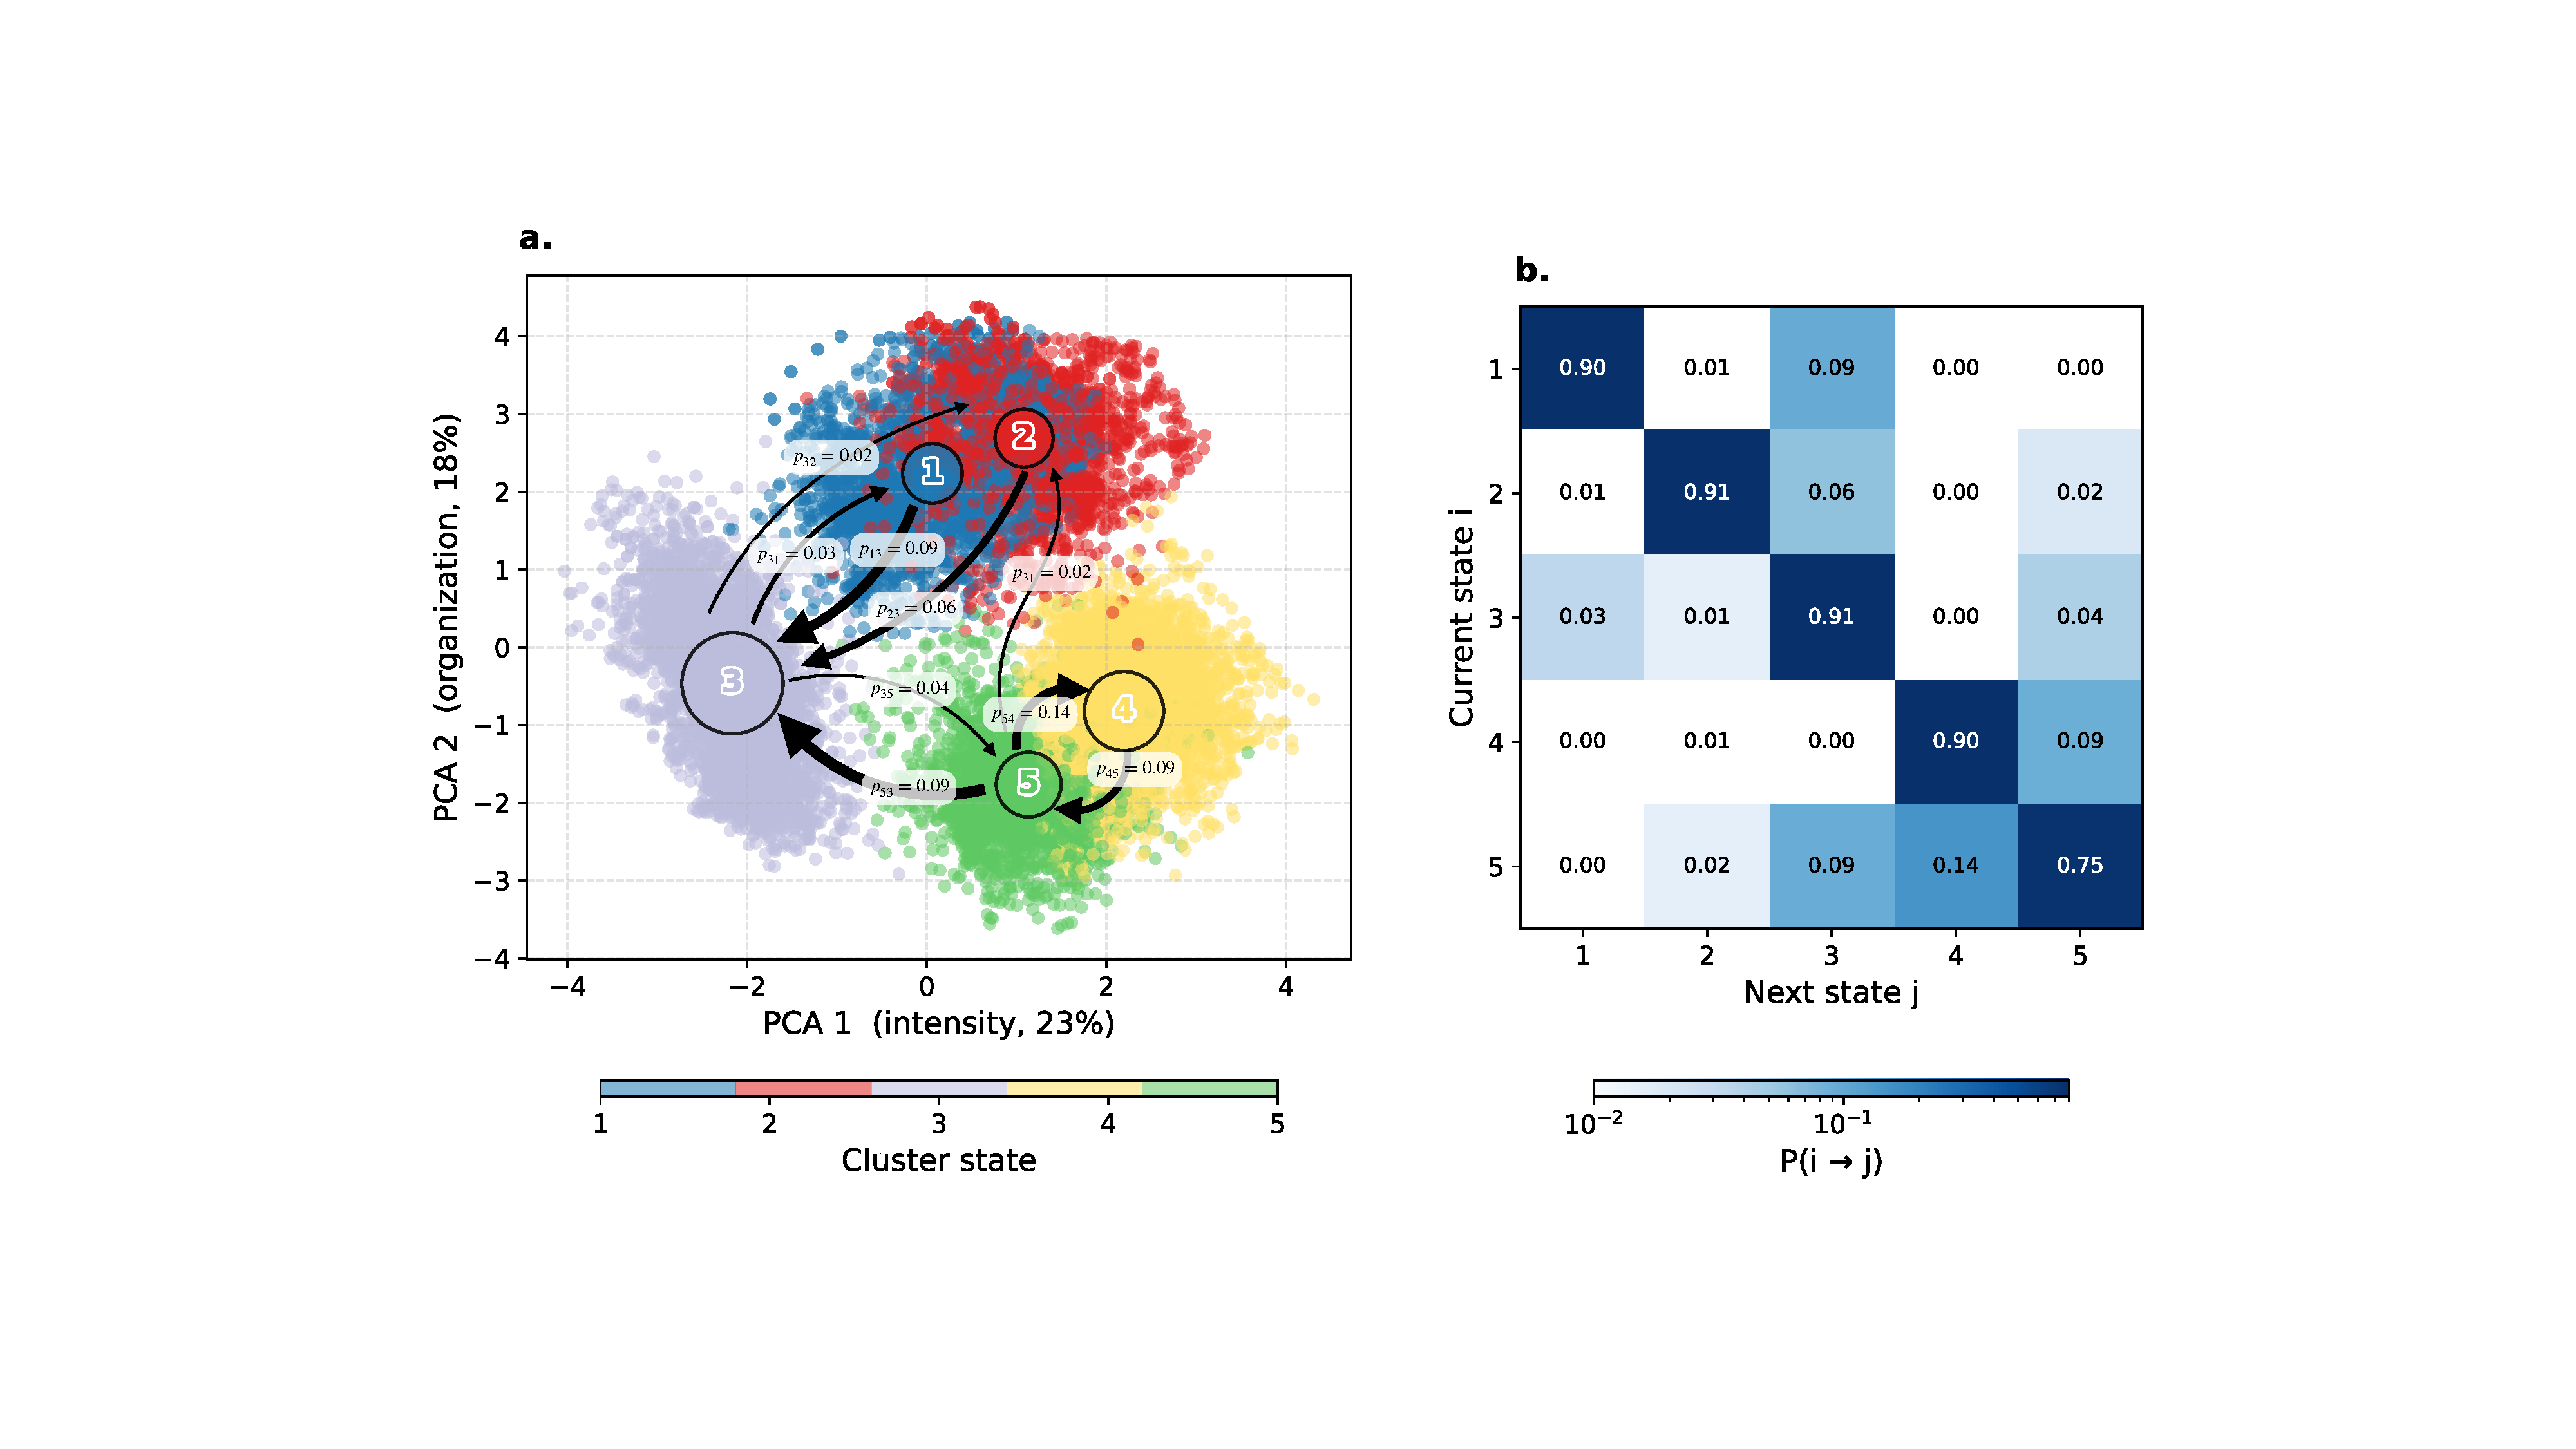
\includegraphics[width=0.92\textwidth]{fig_7_markov_matrix.pdf}
    \caption{\textbf{Markov state dynamics in latent space.} \textbf{(a)} \DIFdelbeginFL \DIFdelFL{Latent space }\DIFdelendFL \DIFaddbeginFL \DIFaddFL{Latent-space }\DIFaddendFL visualization\DIFdelbeginFL \DIFdelFL{with the inferred Markov chain overlaid. The size of }\DIFdelendFL \DIFaddbeginFL \DIFaddFL{; }\DIFaddendFL each state node is \DIFdelbeginFL \DIFdelFL{proportional to }\DIFdelendFL \DIFaddbeginFL \DIFaddFL{sized by }\DIFaddendFL its \DIFdelbeginFL \DIFdelFL{asymptotic (}\DIFdelendFL stationary \DIFdelbeginFL \DIFdelFL{) }\DIFdelendFL probability\DIFdelbeginFL \DIFdelFL{, and arrows indicate transition probabilities between states}\DIFdelendFL . \textbf{(b)} Transition matrix \DIFdelbeginFL \DIFdelFL{describing the dynamics of convection }\DIFdelendFL for the given shear. Two coupled blocks, separated by state~3, form the organized (states~1--2) and unorganized (states~4--5) regimes.}
    \label{fig:markov_matrix}
\end{figure*}

The matrix $\mathbf{T}$ is strongly diagonally \DIFdelbegin \DIFdel{dominated, indicating that the system tends to persist within a given }\DIFdelend \DIFaddbegin \DIFadd{dominant and sparse: the system persists within a }\DIFaddend state over several \DIFdelbegin \DIFdel{time steps. Moreover, the matrix is sparse, }\DIFdelend \DIFaddbegin \DIFadd{steps, }\DIFaddend with only a \DIFdelbegin \DIFdel{limited number of }\DIFdelend \DIFaddbegin \DIFadd{few }\DIFaddend preferred transitions between states\DIFdelbegin \DIFdel{, suggesting constrained pathways in state space}\DIFdelend .

To \DIFdelbegin \DIFdel{further }\DIFdelend characterize the dynamics, we \DIFdelbegin \DIFdel{perform a spectral decomposition of }\DIFdelend \DIFaddbegin \DIFadd{spectrally decompose }\DIFaddend $\mathbf{T}$. \DIFdelbegin \DIFdel{Because $\mathbf{T}$ is }\DIFdelend \DIFaddbegin \DIFadd{Being }\DIFaddend stochastic, it admits a unit eigenvalue $\lambda_1=1$ \DIFdelbegin \DIFdel{. The corresponding }\DIFdelend \DIFaddbegin \DIFadd{whose }\DIFaddend right eigenvector $\boldsymbol{\pi}$ satisfies $\mathbf{T}\boldsymbol{\pi}=\boldsymbol{\pi}$\DIFdelbegin \DIFdel{and defines }\DIFdelend \DIFaddbegin \DIFadd{, }\DIFaddend the stationary distribution\DIFdelbegin \DIFdel{of the Markov chain}\DIFdelend . We obtain
\begin{equation}
\boldsymbol{\pi} =
\begin{bmatrix}
12.9\% & 12.2\% & 37.0\% & 22.7\% & 15.2\%
\end{bmatrix}.
\label{eq:canon}
\end{equation}

The stationary distribution is dominated by state~3 ($37\%$\DIFdelbegin \DIFdel{, suppressed convection}\DIFdelend ), the remaining weight spread across the four active \DIFdelbegin \DIFdel{states---all }\DIFdelend \DIFaddbegin \DIFadd{states, all }\DIFaddend sufficiently populated to constrain the \DIFdelbegin \DIFdel{inferred }\DIFdelend transition statistics.

\DIFdelbegin \DIFdel{We next examine the subdominant eigenvalues and eigenvectors of $\mathbf{T}$. All }\DIFdelend \DIFaddbegin \DIFadd{The }\DIFaddend non-stationary eigenvalues \DIFdelbegin \DIFdel{have imaginary parts at the level of numerical noise }\DIFdelend \DIFaddbegin \DIFadd{are effectively real }\DIFaddend ($|\mathrm{Im}(\lambda_k)|<10^{-3}$)\DIFdelbegin \DIFdel{; the spectrum is effectively real. This indicates that the dominant dynamics cannot be described as simple linear }\DIFdelend \DIFaddbegin \DIFadd{, so the dominant dynamics are not simple }\DIFaddend oscillations in state space.

The leading nontrivial eigenvalue \DIFdelbegin \DIFdel{of the transition matrix }\DIFdelend is $\lambda_2 \approx 0.94$, \DIFdelbegin \DIFdel{indicating }\DIFdelend a highly persistent \DIFdelbegin \DIFdel{dynamical }\DIFdelend mode. The corresponding eigenvector
\begin{equation}
\mathbf{v}_2 =
\begin{bmatrix}
-0.56 & -0.30 & -0.25 & +0.65 & +0.34
\end{bmatrix}
\end{equation}
is unit-norm (the overall sign is arbitrary). A positive $(\mathbf{v}_2)_i$ means state~$i$ is enhanced relative to $\pi_i$ in one phase \DIFdelbegin \DIFdel{of this mode }\DIFdelend and suppressed in the other\DIFdelbegin \DIFdel{; }\DIFdelend \DIFaddbegin \DIFadd{, with }\DIFaddend $|(\mathbf{v}_2)_i|$ \DIFdelbegin \DIFdel{sets the relative size of that deviation across states. Components of opposite sign therefore }\DIFdelend \DIFaddbegin \DIFadd{its relative amplitude; opposite signs }\DIFaddend vary in anti-phase.

The components of $\mathbf{v}_2$ split the chain into two opposite-sign groups, $\{1,2\}$ ($-0.56,\,-0.30$) and $\{4,5\}$ ($+0.65,\,+0.34$); state~3 has the smallest amplitude in this mode ($-0.25$). We interpret these two groups as two convective regimes---\emph{organized} ($\{1,2\}$) and \emph{unorganized} ($\{4,5\}$)---that the chain alternates between on the eigenmode decay time $\tau_2 = -\Delta t / \log|\lambda_2| \approx 172\,\mathrm{min}$. State~3, despite its small amplitude in $\mathbf{v}_2$, carries the dominant stationary occupancy ($\pi_3=37\%$), and nearly every transition between the other four states passes through it (Fig.~\ref{fig:markov_matrix}b)\DIFdelbegin \DIFdel{; it therefore }\DIFdelend \DIFaddbegin \DIFadd{, so it }\DIFaddend functions as the chain's intermediate state\DIFdelbegin \DIFdel{, visited routinely between successive episodes in the other states}\DIFdelend .

The internal dynamics of the two regimes differ. The unorganized regime is a closed oscillation: states~4 and~5 exchange directly and frequently ($T_{4\to 5}=0.09$, $T_{5\to 4}=0.14$). The organized regime is not\DIFdelbegin \DIFdel{. States}\DIFdelend \DIFaddbegin \DIFadd{: states}\DIFaddend ~1 and~2 do not exchange directly ($T_{1\to 2}=T_{2\to 1}=0.01$) \DIFdelbegin \DIFdel{, and they are also separated in time: }\DIFdelend \DIFaddbegin \DIFadd{and are separated in time---}\DIFaddend $200$~min after a state-1 timestep, the \DIFdelbegin \DIFdel{conditional }\DIFdelend probability of being in state~2 is $0.04$, well below the stationary \DIFdelbegin \DIFdel{value }\DIFdelend $\pi_2=0.12$. State\DIFaddbegin \DIFadd{s}\DIFaddend  ~1 \DIFdelbegin \DIFdel{(deep moist ascent, reduced low-level detrainment) andstate}\DIFdelend \DIFaddbegin \DIFadd{and}\DIFaddend ~2 \DIFdelbegin \DIFdel{(mesoscale stratiform-like deep convection) }\DIFdelend therefore appear as independent organized episodes, each returning to state~3 before the next can begin. \DIFdelbegin \DIFdel{Time series of individual }\DIFdelend \DIFaddbegin \DIFadd{Individual }\DIFaddend realizations (Supplemental Material, Fig.~\ref{Sfig:trajectories}) reflect this: organized intervals are dominated by a $3\!\leftrightarrow\!1$ oscillation\DIFdelbegin \DIFdel{with occasional state-2 excursions, while unorganized intervals follow }\DIFdelend \DIFaddbegin \DIFadd{, unorganized intervals by }\DIFaddend the $3\!\leftrightarrow\!5\!\leftrightarrow\!4$ cycle.

The \DIFdelbegin \DIFdel{eigenvalue spectrum just identified }\DIFdelend \DIFaddbegin \DIFadd{spectrum }\DIFaddend makes a quantitative prediction: for a true Markov chain, the autocorrelation of \DIFdelbegin \DIFdel{every }\DIFdelend \DIFaddbegin \DIFadd{each }\DIFaddend state's occupancy \DIFdelbegin \DIFdel{must be }\DIFdelend \DIFaddbegin \DIFadd{is }\DIFaddend a sum of exponentials with \DIFdelbegin \DIFdel{the }\DIFdelend decay times $\tau_k = -\Delta t / \log|\lambda_k|$\DIFdelbegin \DIFdel{. We next test this prediction directly }\DIFdelend \DIFaddbegin \DIFadd{, which we now test }\DIFaddend against the empirical autocorrelations\DIFdelbegin \DIFdel{, identifying which states deviate from Markovian behavior and how those deviations reveal internal feedbacks such as cold-pool memory}\DIFdelend .

\section{Markovianity assessment and internal feedbacks}
\label{sec:markov}

We now ask whether the five-state chain is \DIFdelbegin \DIFdel{self-contained---whether }\DIFdelend \DIFaddbegin \DIFadd{self-contained: whether }\DIFaddend the state at time $t$ alone determines the distribution at $t+\tau$. Departures \DIFdelbegin \DIFdel{from this Markov property }\DIFdelend identify slow internal \DIFdelbegin \DIFdel{processes (moisture }\DIFdelend \DIFaddbegin \DIFadd{processes---moisture }\DIFaddend memory, cold pools, mesoscale \DIFdelbegin \DIFdel{organization) that }\DIFdelend \DIFaddbegin \DIFadd{organization---that }\DIFaddend the partition does not resolve. The question is long-standing: classical \DIFdelbegin \DIFdel{convective }\DIFdelend parameterizations assume instantaneous quasi-equilibrium adjustment \cite{zhang2003convective, bechtold2014representing}, while \DIFdelbegin \DIFdel{more recent schemes introduce }\DIFdelend \DIFaddbegin \DIFadd{recent schemes add }\DIFaddend explicit memory variables \DIFdelbegin \DIFdel{to capture }\DIFdelend \DIFaddbegin \DIFadd{for }\DIFaddend lagged responses \cite{piriou2007approach, gerard2009cloud, mapes2011parameterizing, hwong2023assessing}.

\emph{Indicator autocorrelation.}---Defining the occupancy indicator $I_i(t) = \mathbf{1}[X_t = i]$ and its normalized autocorrelation
\begin{equation}
C_i(\tau) =
\frac{\mathbb{E}\!\left[(I_i(t)-\pi_i)(I_i(t+\tau)-\pi_i)\right]}{\mathbb{E}\!\left[(I_i(t)-\pi_i)^2\right]},
\end{equation}
a discrete-time Markov chain with transition matrix $\mathbf{T}$ and stationary distribution $\boldsymbol{\pi}$ admits the closed form \cite{souza2024representing}
\begin{equation}
C_i(\tau) \;=\; \frac{T^\tau_{ii} - \pi_i}{1-\pi_i}
\;=\; \sum_{\alpha=2}^K A_\alpha^{(i)}\, \lambda_\alpha^\tau,
\label{eq:autocor}
\end{equation}
a superposition of exponentially decaying modes set by the eigenvalues $\lambda_\alpha$ of $\mathbf{T}$, with \DIFdelbegin \DIFdel{state-dependent }\DIFdelend amplitudes $A_\alpha^{(i)} = (\mathbf{v}_\alpha)_i (\mathbf{w}_\alpha)_i / (1-\pi_i)$ \DIFdelbegin \DIFdel{, where }\DIFdelend \DIFaddbegin \DIFadd{(}\DIFaddend $\mathbf{v}_\alpha$\DIFdelbegin \DIFdel{and }\DIFdelend \DIFaddbegin \DIFadd{, }\DIFaddend $\mathbf{w}_\alpha$ \DIFdelbegin \DIFdel{are }\DIFdelend the right and left eigenvectors\DIFdelbegin \DIFdel{of $\mathbf{T}$ (}\DIFdelend \DIFaddbegin \DIFadd{; }\DIFaddend derivation in the Supplemental Material). Departures from \DIFdelbegin \DIFdel{this prediction }\DIFdelend \DIFaddbegin \DIFadd{it }\DIFaddend quantify residual memory not encoded by the partition.

\emph{Memory beyond Markov in the convection-active states.}---In Fig.~\ref{fig:autocorrelation}a, the empirical autocorrelations decrease and fall below $0.2$ within the lag window, in line with the Markov prediction of Eq.~\eqref{eq:autocor}---except for the organized state~1 (blue) and the active-unorganized state~4 (yellow), which stay elevated, well above their predictions; state~3 (suppressed convection) tracks its prediction most closely. This distinction matters: a state can be \emph{sustained} \DIFdelbegin \DIFdel{(long dwell times) and }\DIFdelend \DIFaddbegin \DIFadd{yet }\DIFaddend still \emph{Markovian} if its diagonal $T_{ii}$ \DIFdelbegin \DIFdel{alone }\DIFdelend explains the persistence; states~1 and~4 \DIFdelbegin \DIFdel{are sustained }\DIFdelend \DIFaddbegin \DIFadd{persist }\DIFaddend \emph{beyond} what $T_{ii}$ predicts, \DIFdelbegin \DIFdel{indicating that }\DIFdelend \DIFaddbegin \DIFadd{so }\DIFaddend an internal degree of freedom \DIFdelbegin \DIFdel{not represented in }\DIFdelend \DIFaddbegin \DIFadd{absent from }\DIFaddend the partition is keeping them alive.

\emph{Cold pools partly close the gap.}---Cold pools---masses of cold, dense air \DIFdelbegin \DIFdel{that form }\DIFdelend \DIFaddbegin \DIFadd{formed }\DIFaddend below convective clouds \DIFdelbegin \DIFdel{through }\DIFdelend \DIFaddbegin \DIFadd{by }\DIFaddend rain evaporation and \DIFdelbegin \DIFdel{are }\DIFdelend a key control on squall-line organization \cite{rotunno1988theory, houze1977structure, tompkins2001coldpools, abramian2022shear}---are a natural \DIFdelbegin \DIFdel{candidate }\DIFdelend carrier of this memory: they outlast the downdrafts that generate them and trigger or suppress \DIFdelbegin \DIFdel{new }\DIFdelend convection at their gust fronts \cite{torri2015mechanisms}, \DIFdelbegin \DIFdel{so they can sustain }\DIFdelend \DIFaddbegin \DIFadd{sustaining }\DIFaddend an organized state beyond what the instantaneous partition records. The hypothesis is testable: if cold pools carry the memory, \DIFdelbegin \DIFdel{then }\DIFdelend knowing the cold-pool field at the starting time should make the subsequent state~1 dynamics more \DIFdelbegin \DIFdel{Markovian---faster autocorrelation decay, closer to the Markov prediction}\DIFdelend \DIFaddbegin \DIFadd{Markovian}\DIFaddend . To test this we introduce an indicator that picks out state~1 timesteps with a high cold pool,
\begin{equation}
J_1^\star(t) \;=\; \mathbf{1}\!\left[X_t = 1 \,\text{ and }\, \mathrm{CP}(t) > \mathrm{CP}_\star\right],
\end{equation}
where $\mathrm{CP}(t)$ is a cold-pool index---the total area covered by cold pools at time $t$, normalized by its temporal mean (Supplemental Material)---and $\mathrm{CP}_\star$ is its 75th percentile. The cold-pool-conditioned state~1 survival is then the expected state~1 occupancy a lag $\tau$ later, averaged over the timesteps selected by $J_1^\star$:
\begin{equation}
S^{(\mathrm{CP})}_1(\tau) \;=\; \mathbb{E}\!\left[\,I_1(t+\tau) \,\big|\, J_1^\star(t) = 1\,\right].
\end{equation}
We then rescale to autocorrelation form via $C^{(\mathrm{CP})}_1(\tau) = (S^{(\mathrm{CP})}_1(\tau) - \pi_1)/(1-\pi_1)$ for comparison with panel~(a). The condition is applied \emph{only at the starting time}; the trajectory is free \DIFdelbegin \DIFdel{thereafter---holding it throughout would truncate the survival artificially }\DIFdelend \DIFaddbegin \DIFadd{thereafter }\DIFaddend (Supplemental Material). The conditioned curve (Fig.~\ref{fig:autocorrelation}b, dashed) sits between the unconditional empirical curve (solid) and the Markov reference (dotted), closing roughly $30\%$ of the gap at a $200$~min lag: more Markovian, but not fully.

\emph{Cold pools are part---but not all---of the hidden memory.}---The unclosed portion of the gap implicates other slow \DIFdelbegin \DIFdel{internal variables: mesoscale }\DIFdelend \DIFaddbegin \DIFadd{variables---mesoscale }\DIFaddend moisture pooling \cite{mapes2011parameterizing}, cloud-cluster geometry \cite{hwong2023assessing}, \DIFdelbegin \DIFdel{and }\DIFdelend free-tropospheric \DIFdelbegin \DIFdel{humidity all evolve on the relevant }\DIFdelend \DIFaddbegin \DIFadd{humidity---evolving on similar }\DIFaddend time scales. Two caveats apply: $\mathrm{CP}(t)$ collapses spatial structure into a scalar, and stratifying by \DIFdelbegin \DIFdel{$\mathrm{CP}(t)$ }\DIFdelend \DIFaddbegin \DIFadd{it }\DIFaddend inherits some lifecycle-stage dependence; Supplemental Material sensitivity tests \DIFdelbegin \DIFdel{(per-cold-pool diagnostic and entry-conditional survival anchored at state~1 entries) }\DIFdelend are consistent with the closure reported here. A definitive identification \DIFdelbegin \DIFdel{of the dominant carrier }\DIFdelend would require re-training the encoder with explicit cold-pool inputs, \DIFdelbegin \DIFdel{which we leave }\DIFdelend \DIFaddbegin \DIFadd{left }\DIFaddend to future work.

\begin{figure*}[t]
    \centering
    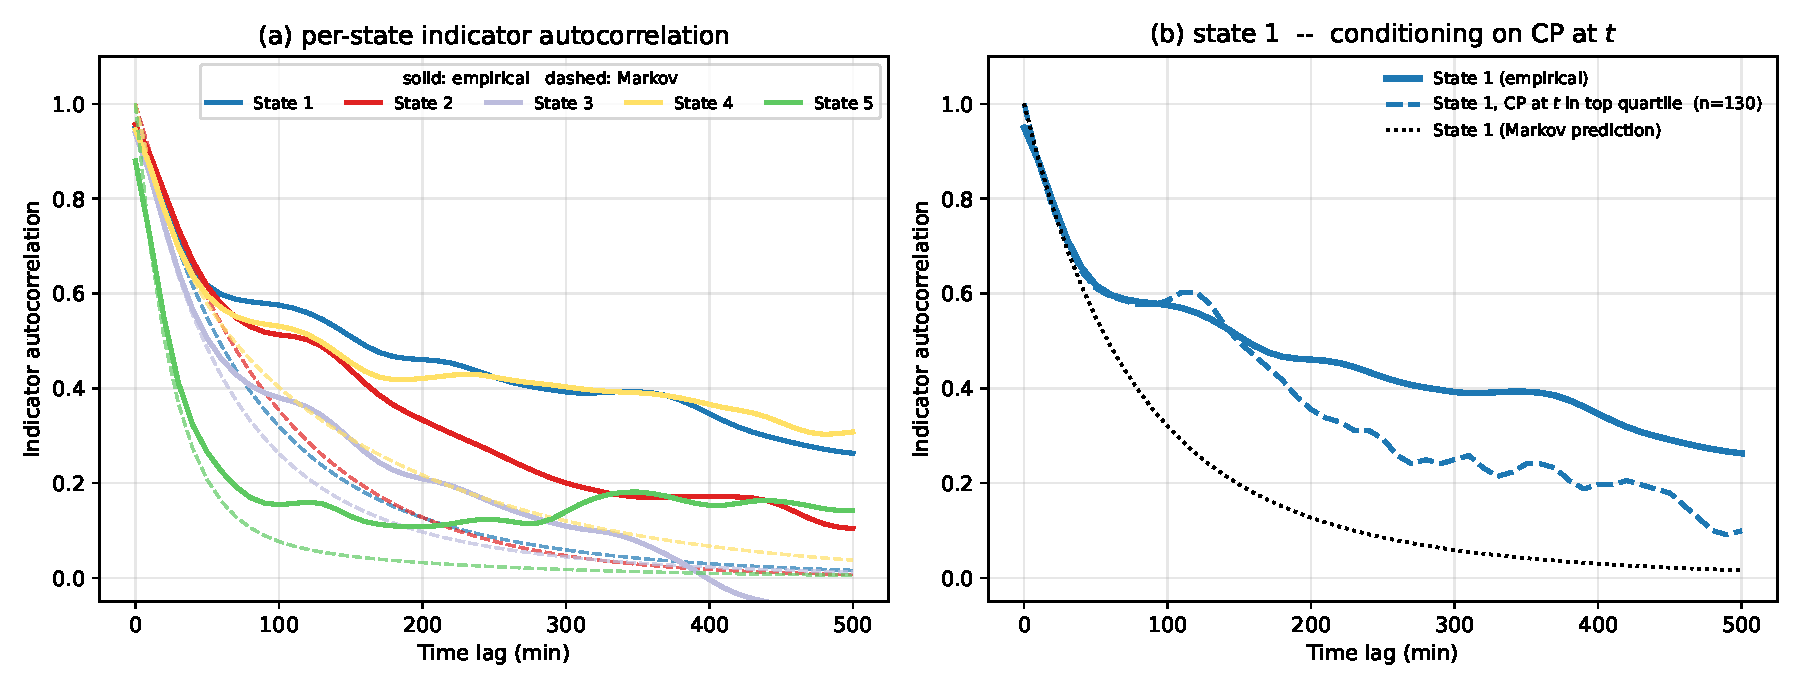
\includegraphics[width=0.9\textwidth]{fig9bis_markovianity_coldpools.pdf}
    \caption{\textbf{Markovianity assessment.} \textbf{(a)}~Per-state indicator autocorrelations (solid) and \DIFdelbeginFL \DIFdelFL{their }\DIFdelendFL Markov predictions (dashed, same colour); states~1 and~4 sit \DIFdelbeginFL \DIFdelFL{visibly }\DIFdelendFL above their predictions, the others track theirs\DIFdelbeginFL \DIFdelFL{closely}\DIFdelendFL . \textbf{(b)}~State-1 autocorrelation: empirical (solid\DIFdelbeginFL \DIFdelFL{blue}\DIFdelendFL ), Markov prediction (dotted\DIFdelbeginFL \DIFdelFL{black}\DIFdelendFL ), and empirical conditioned on $\mathrm{CP}(t)>\mathrm{CP}_\star$ at the starting time (dashed\DIFdelbeginFL \DIFdelFL{blue}\DIFdelendFL ), \DIFdelbeginFL \DIFdelFL{which closes }\DIFdelendFL \DIFaddbeginFL \DIFaddFL{closing }\DIFaddendFL $\sim$30\% of the \DIFdelbeginFL \DIFdelFL{empirical--Markov }\DIFdelendFL gap at a 200~min lag.}
    \label{fig:autocorrelation}
\end{figure*}

\section{Discussion}

Convection varies widely even under a fixed forcing, yet this variability is structured, not random. \DIFdelbegin \DIFdel{We represented the flow with isentropic analysis and encoded }\DIFdelend \DIFaddbegin \DIFadd{Casting the flow in isentropic coordinates and encoding }\DIFaddend it into a low-dimensional latent space, \DIFdelbegin \DIFdel{where its evolution reduces }\DIFdelend \DIFaddbegin \DIFadd{we reduced its evolution }\DIFaddend to a Markov chain over \DIFdelbegin \DIFdel{a few discrete states . Five states proved enough to }\DIFdelend \DIFaddbegin \DIFadd{five discrete states that }\DIFaddend recover physically meaningful \DIFdelbegin \DIFdel{convective regimesand to follow the trajectories convection takes between them. This }\DIFdelend \DIFaddbegin \DIFadd{regimes. The }\DIFaddend chain is nearly memoryless\DIFdelbegin \DIFdel{, with }\DIFdelend \DIFaddbegin \DIFadd{: }\DIFaddend a single slow eigenmode ($\lambda_2\approx0.94$, $\tau_2\approx172$~min) \DIFdelbegin \DIFdel{that alternates two regimes, }\DIFdelend \DIFaddbegin \DIFadd{alternates }\DIFaddend organized and unorganized \DIFdelbegin \DIFdel{, }\DIFdelend \DIFaddbegin \DIFadd{regimes }\DIFaddend around a dominant suppressed background ($\pi_3=37\%$)\DIFdelbegin \DIFdel{; two competing routes emerge, a }\DIFdelend \DIFaddbegin \DIFadd{, with two competing routes---a }\DIFaddend direct ascent into deep convection and a slower drift through weakly organized phases. \DIFdelbegin \DIFdel{The framework's }\DIFdelend \DIFaddbegin \DIFadd{Its }\DIFaddend distinctive feature is \DIFdelbegin \DIFdel{that }\DIFdelend \DIFaddbegin \DIFadd{diagnostic: }\DIFaddend departures from Markovianity \DIFdelbegin \emph{\DIFdel{diagnose}} %DIFAUXCMD
\DIFdel{what the discrete partition omits: states~1 and~4 persist beyond their Markov prediction}\DIFdelend \DIFaddbegin \DIFadd{reveal what the partition omits}\DIFaddend , and conditioning on cold-pool intensity closes $\sim$30\% of \DIFdelbegin \DIFdel{that }\DIFdelend \DIFaddbegin \DIFadd{the }\DIFaddend gap at a $200$~min lag, identifying cold pools as one measurable carrier of the hidden memory.

These results describe a single \DIFdelbegin \DIFdel{, idealized forcing---fixed vertical shear in radiative--convective equilibrium---and }\DIFdelend \DIFaddbegin \DIFadd{idealized forcing, and }\DIFaddend the simplicity of the latent space may partly reflect that control\DIFdelbegin \DIFdel{: a more variable or transient forcing could populate a higher-dimensional space with more states and stronger non-Markovianity. Testing this is the natural next step. }\DIFdelend \DIFaddbegin \DIFadd{. }\DIFaddend Because the transition matrix \DIFdelbegin \DIFdel{is a function of }\DIFdelend \DIFaddbegin \DIFadd{depends on }\DIFaddend the forcing, repeating the construction across shear regimes---weak (popcorn), moderate, strong (supercritical squall lines)\DIFdelbegin \DIFdel{---turns }\DIFdelend \DIFaddbegin \DIFadd{---would turn }\DIFaddend convective organization into a measurable dynamical observable\DIFdelbegin \DIFdel{: under stronger shear the }\DIFdelend \DIFaddbegin \DIFadd{, with }\DIFaddend organized-state persistence $T_{ii}$ and eigenmode time scales \DIFdelbegin \DIFdel{should lengthen, and the direct route into deep convection should dominate. Sharper internal descriptors---cold-pool age, gust-front strength, mesoscale moisture, or cluster geometry---should each close more of the memory gap, every increment naming another slow variable a memory-aware parameterization must track}\DIFdelend \DIFaddbegin \DIFadd{lengthening under stronger shear}\DIFaddend .

\section*{Data and Code Availability}

The idealized squall-line SAM simulations (27 days at 2-minute resolution, with 1D, 2D, and 3D outputs) are available via Globus (link to be provided). All code is openly available at \url{https://github.com/sososquirrel/troposwhere}, including the model implementation and the scripts to reproduce all figures. Full methods---simulation setup, isentropic preprocessing, model architecture, training, and sensitivity tests---are given in the Supplemental Material.

\section*{Acknowledgments}

We are grateful to Juan Nathanael and Carla Roesch for discussions on Koopman operators, and to Fabrizio Falasca and Matthieu Blanke for recommendations on the dynamical systems literature. We also thank Sara Shamekh, Zhe Feng, Xingchao Chen, and the WACCEM project team for valuable discussions throughout the course of this study. We thank Koichi Sakaguchi and Huancui Hu for their internal review and constructive feedback. Portions of the manuscript were rephrased with the assistance of ChatGPT (OpenAI) for language editing, and Claude (Anthropic) assisted with aspects of code development and cleaning; all scientific ideas, analysis, and conclusions were developed by the authors. 

This study is supported by Office of Science, U.S. Department of Energy (DOE) Biological and Environmental Research as part of the Regional and Global Model Analysis program area through the Water Cycle: Modeling of Circulation, Convection, and Earth System Mechanisms (WACCEM) scientific focus area. S.A. designed the research, performed the simulations, developed the methods and code, and wrote the manuscript. O.P. contributed to the methodological development and the code and participated in the analysis and discussions. L.R.L. and P.G. contributed to improving the analysis and interpretation.

\bibliographystyle{apsrev4-2}
\bibliography{biblio}

\end{document}
